\appendix

% -------------------------------
% Section: Experteninterview
% -------------------------------
\section{Experteninterview} \label{app:interview}

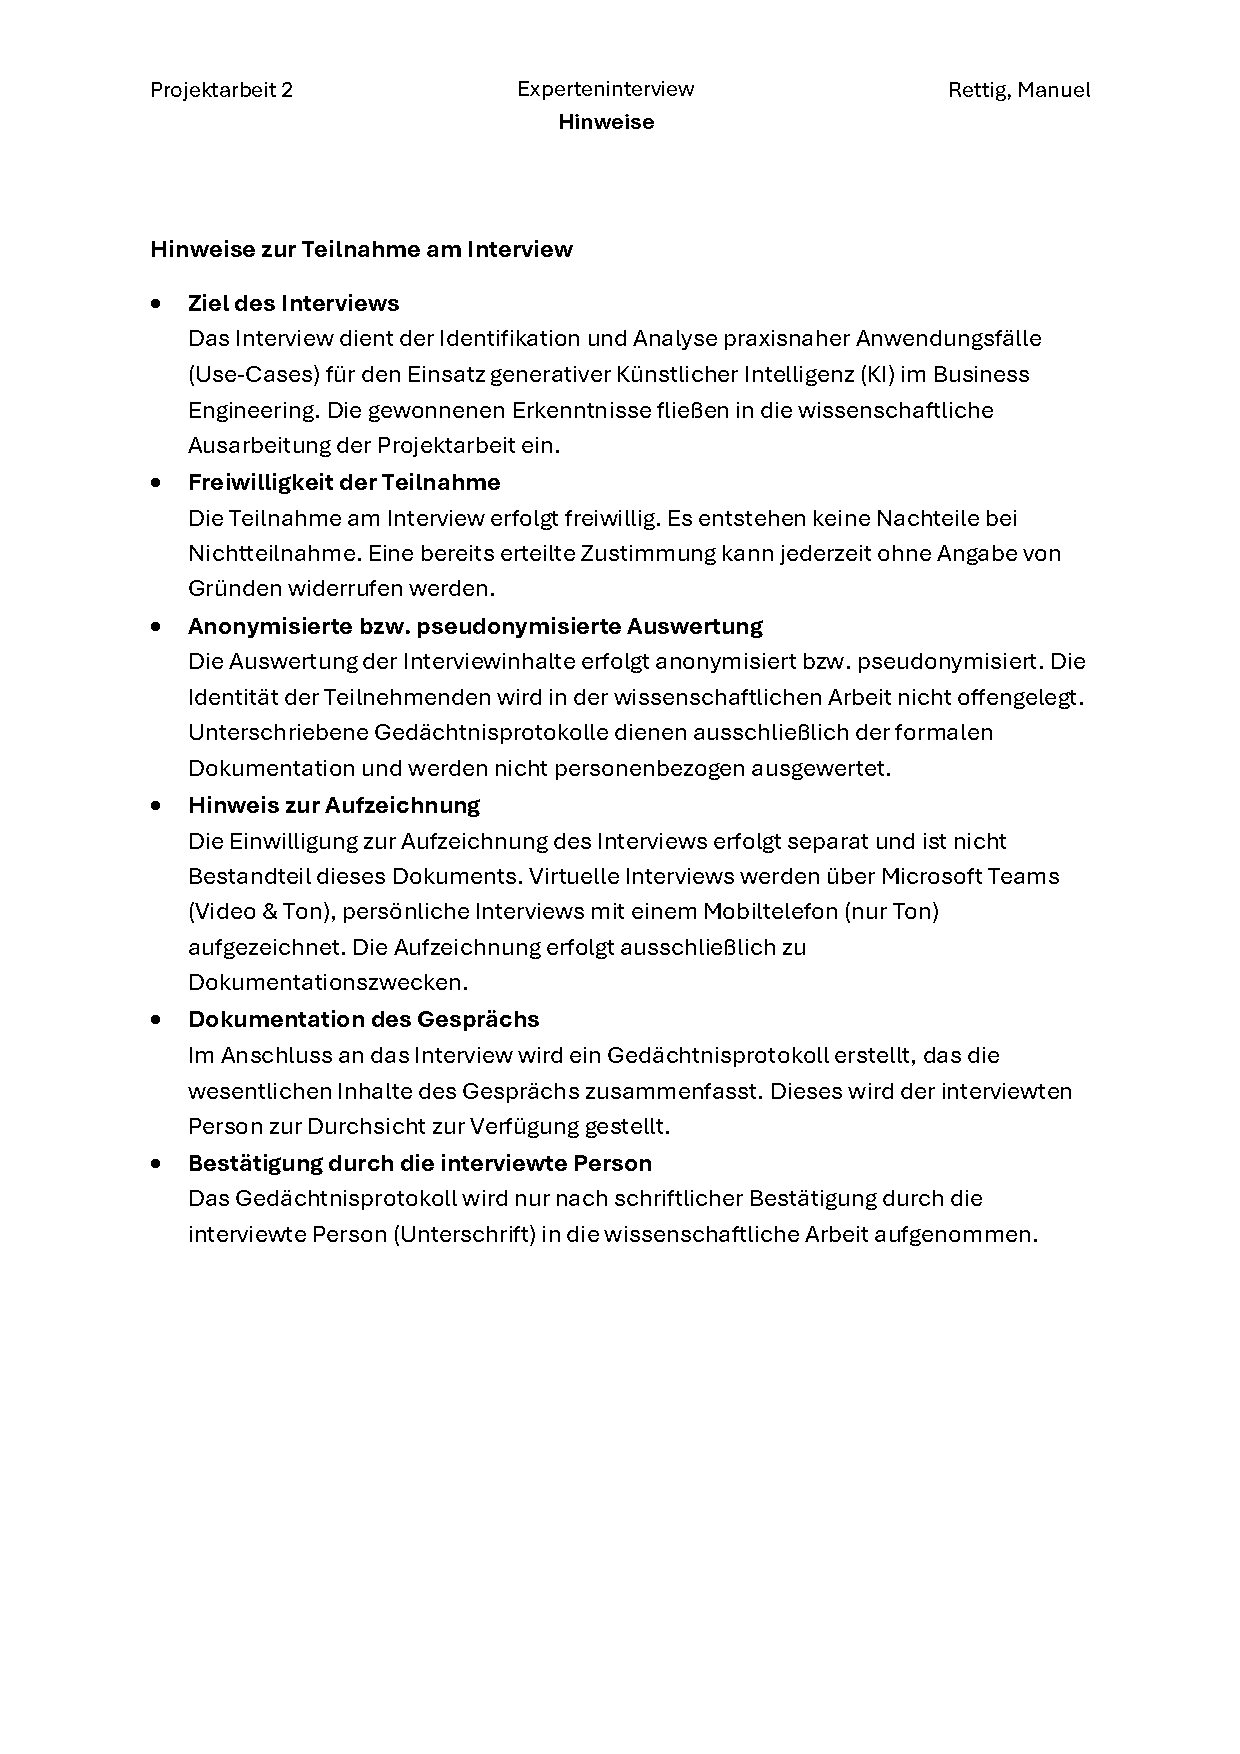
\includepdf[
  scale=0.7,
  frame,
  pagecommand={
    \thispagestyle{fancy}%
    \subsection{Interviewleitfaden}%
    \label{app:leitfaden}%
  }
]{Interview_Hinweise.pdf}

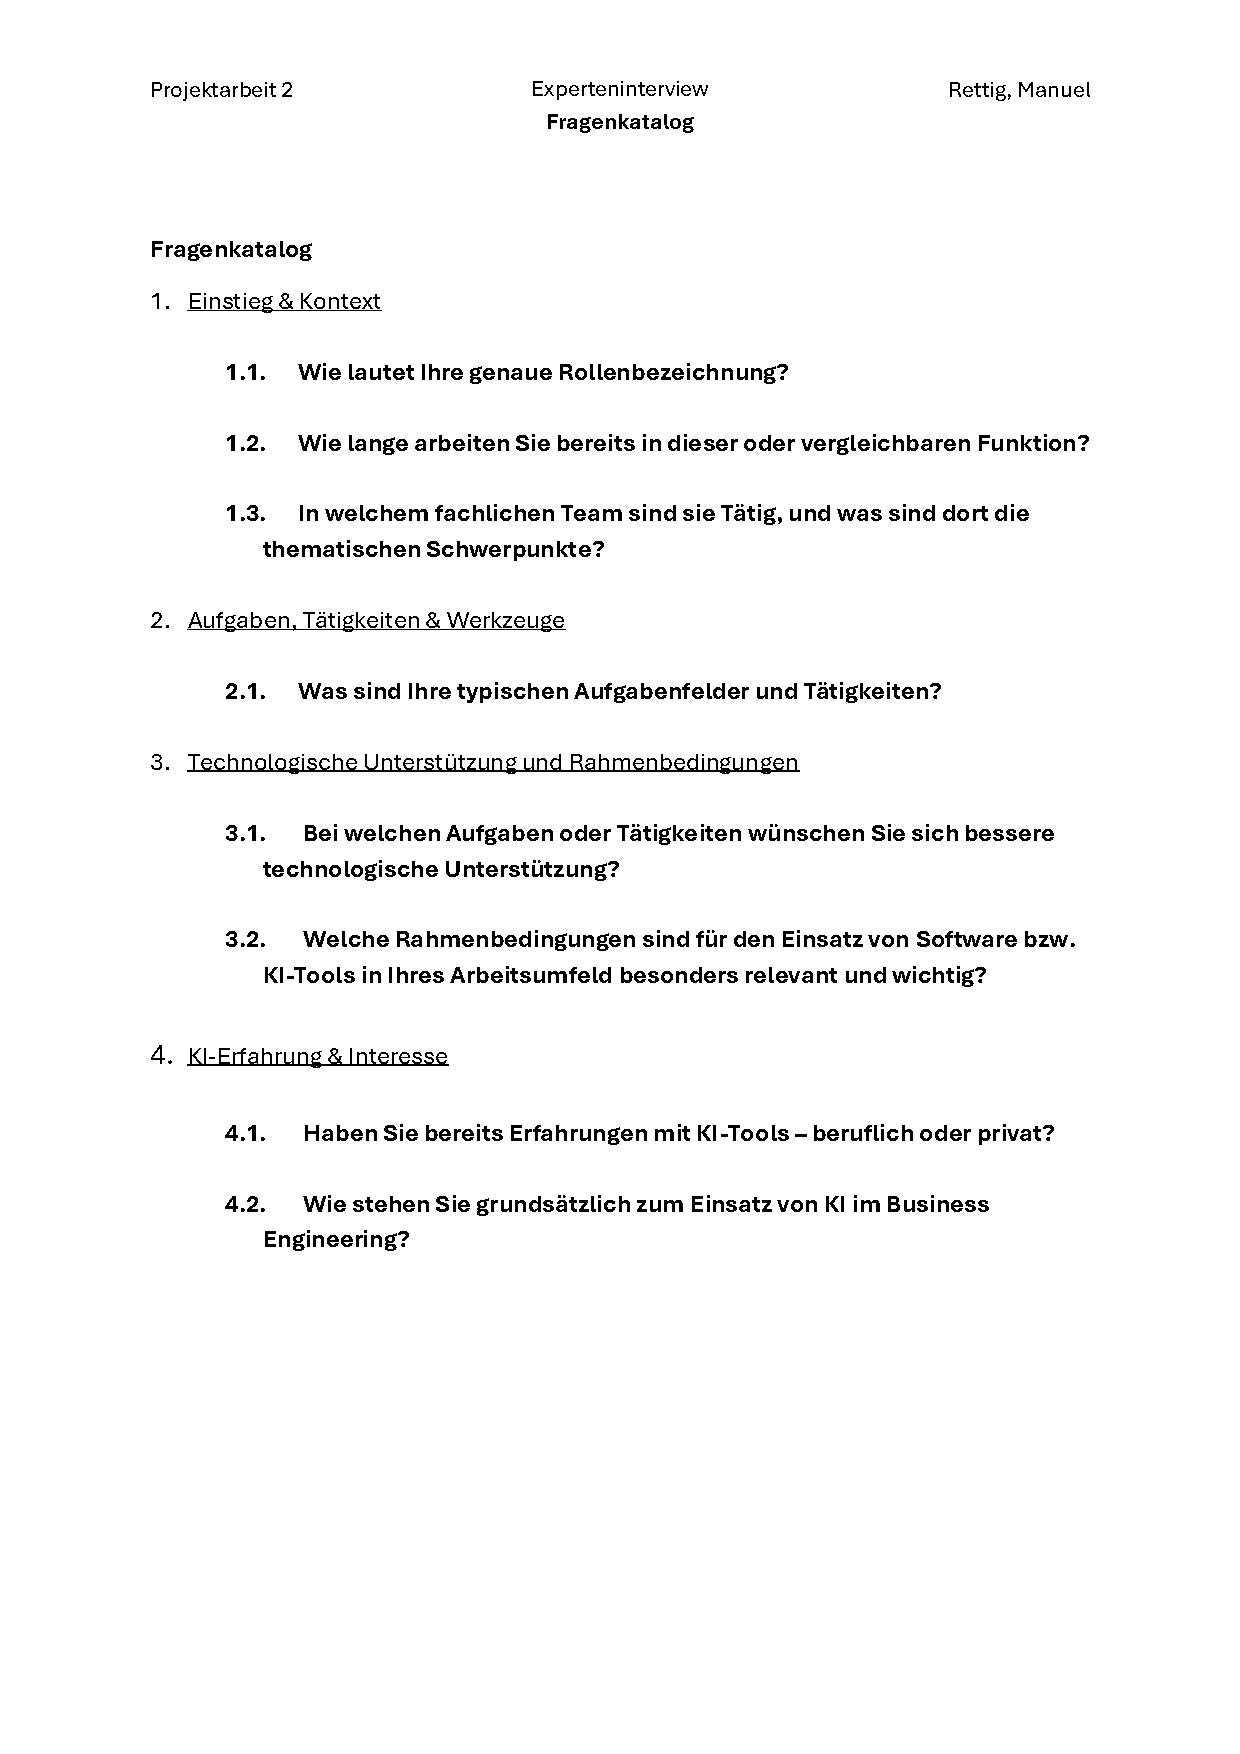
\includepdf[
  scale=0.7,
  frame,
  pagecommand={}
]{Interview_Fragenkatalog.pdf}

% \newcommand{\includeinterview}[2]{%
%   \includepdf[
%     pages=1,
%     scale=0.7,
%     frame,
%     pagecommand={
%       \thispagestyle{fancy}%
%       \subsection{Interviewprotokoll E#1}%
%       \label{app:interview#1}%
%     }
%   ]{Protokoll_#2.pdf}
%   \includepdf[
%     pages=2-,
%     scale=0.7,
%     frame,
%     pagecommand={}
%   ]{Protokoll_#2.pdf}
% }

% \includeinterview{1}{E1}

\subsection{Interviewprotokoll 1} \label{app:interview1}
Aus Vertraulichkeitsgründen nicht enthalten.

\newpage
\section{Hilfsmittelverzeichnis}

\begin{table}[H]
  \scriptsize
  \begin{tabularx}{\textwidth}{|P{0.2\textwidth}|P{0.14\textwidth}|X|P{0.16\textwidth}|}
    \hline
    \textbf{Arbeitsschritt} &
    \textbf{KI-Systeme} &
    \textbf{Beschreibung der Verwendungsweise} &
    \textbf{Betroffene Teile der Arbeit} \\
    \hline
    Generierung von Ideen und Konzeption & ChatGPT, MS-Copilot & Diskussion und regelmäßiges Feedback zur Schärfung des Aufbaus und Konzepts & Gesamte Arbeit \\
    \hline
    Literatursuche & Perplexity.ai & Erste thematische Recherchen zur Orientierung im Forschungsfeld & Kapitel 2, 5 \\
    \hline
    Literaturanalyse & ChatGPT, MS-Copilot & Unterstützung bei Strukturierung und Verdichtung zentraler Aussagen & Kapitel 2, 5 \\
    \hline
    Auswahl von Methoden und Modellen & ChatGPT, MS-Copilot & Feedback und Diskussionen zur methodischen Vorgehensweisen basierend auf eigenen Ideen und Ansätze & Kapitel 3 \\
    \hline
    Datensammlung und -analyse & ChatGPT, MS-Copilot & Unterstützung bei Kategorisierung und Zusammenfassung der Interviewprotokolle & Kapitel 4 \\
    \hline
    Interpretation und Validierung & ChatGPT, MS-Copilot & Reflexions- und Interpretationshilfe durch Zusammenfassung von Argumentationen & Kapitel 4-7 \\
    \hline
    Strukturierung des Texts & ChatGPT, MS-Copilot & Unterstützung bei Gliederung und Formulierung von Übergängen & Gesamte Arbeit \\
    \hline
    Formulierung des Texts & ChatGPT & Sprachliche Verfeinerung einzelner Absätze auf Basis vorliegender Inhalte & Gesamte Arbeit \\
    \hline
  \end{tabularx}
\end{table}